
\documentclass[10pt]{article} % For LaTeX2e
% \usepackage{tmlr}
% If accepted, instead use the following line for the camera-ready submission:
% \usepackage[accepted]{tmlr}
% To de-anonymize and remove mentions to TMLR (for example for posting to preprint servers), instead use the following:
\usepackage[preprint]{tmlr}

% Optional math commands from https://github.com/goodfeli/dlbook_notation.
\input{math_commands.tex}

\usepackage{hyperref}
\usepackage{url}
\usepackage{graphicx} % Required for inserting images
\usepackage{amsmath} 
\usepackage{booktabs}
\usepackage{multirow}
\usepackage{amsfonts}
\usepackage{natbib}

\title{Improving Quality of Service in Network Routing  with Graph Neural Network-Based Multi-Agent Reinforcement Learning}

% Authors must not appear in the submitted version. They should be hidden
% as long as the tmlr package is used without the [accepted] or [preprint] options.
% Non-anonymous submissions will be rejected without review.

\author{\name Dean Verrell Matalino Ariefin \email dean.ariefin.25@ucl.ac.uk \\
      \addr Department of Electronic and Electrical Engineering\\
      University College London}

% The \author macro works with any number of authors. Use \AND 
% to separate the names and addresses of multiple authors.

\newcommand{\fix}{\marginpar{FIX}}
\newcommand{\new}{\marginpar{NEW}}

\def\month{MM}  % Insert correct month for camera-ready version
\def\year{YYYY} % Insert correct year for camera-ready version
\def\openreview{\url{https://openreview.net/forum?id=XXXX}} % Insert correct link to OpenReview for camera-ready version


\begin{document}


\maketitle

\begin{abstract}
An interconnection network (Internet) is a group of networks consisting of nodes carrying traffic between multiple sites. As traffic demand increases rapidly, network routing protocols must deliver efficient and adaptive solutions for packet transmission. This study introduces a new routing protocol for the Internet that combines Multi-Agent Reinforcement Learning (MARL) with Graph Neural Networks (GNN) to improve Quality of Service (QOS). In this approach, each network node is modeled as an autonomous agent that utilizes a GNN-based state to capture both local and global network environment data. Nodes use a centralized training and decentralized execution model to optimize routing decision strategies. The protocol is assessed using NS-3 simulations to measure Quality of Service performance. Under overload traffic, the approach outperforms the Open Shortest Path First (OSPF) routing protocol on two of the three evaluation networks, reducing packet loss from $14.1$--$27.3\%$ to $3.4$--$10.6\%$ and delay from $19.7$--$21.4$\,ms to $17.1$--$18.1$\,ms. The evaluation also shows the approach lowers maximum link utilization from 95.6–97.3\% to 65.5–66.3\% in the feasible regimes. Integrating MARL with GNNs enhances the quality of service on network routing. This approach allows networks to learn and adapt across different network topologies, providing efficient solutions for real-world applications.
\end{abstract}

\section{Introduction} 
%Describe OSPF
Interconnection networks consist of groups of nodes that carry aggregated traffic across multiple sites and capacity links. The task of network routing is to transmit data between sources and destinations. Within the same domain, this type of network is called an intra-domain network. Intra-domain networks require routing protocols to facilitate packet transmission between nodes. A widely used protocol in these networks is the Open Shortest Path First (OSPF) routing protocol \citep{rfc2328}. OSPF is a link-state protocol that detects topological changes within the Autonomous System (AS), routes packets based on the IP header, and determines the optimal path using Dijkstra’s algorithm.

%Describe OSPF Limitation
OSPF has limited flexibility in intra-domain routing. The authoritative OSPF standard uses a single configuration cost that restricts protocol adjustments to the link weights \citep{rfc2328}. OSPF does not account for the real-time condition of links between nodes. The protocol ignores real-time load and capacity when using static weights. These limitations can create network congestion \citep{1039866}. As a result, intra-domain routing faces challenges in maintaining connectivity because standard OSPF offers limited traffic-engineering capability.

%Describe Research Gap  
As network traffic demand grows, there is a need for better network routing solutions. Multi-Agent Reinforcement Learning with a Graph Neural Network (GNN) method has recently been applied to dynamic routing in mobile ad-hoc networks  \citep{11134361}. However, existing research mainly focuses on wireless, mobile, and topology-varying environments. Their applicability to intra-domain routing, where routing is driven by capacity and traffic, remains unexplored. Furthermore, other previous studies also evaluated routing performance using synthetic traffic rather than real network demand.

%Describe Proposed Approach
To address these gaps, this work applies and adapts Multi-Agent Reinforcement Learning with a Graph Neural Network (GNN) backbone to intra-domain telecommunication backbone routing. Reinforcement Learning is a machine learning paradigm in which agents learn optimal actions through a system of rewards and punishment \citep{SHAKARAMI2020107496}. Multi-agent Reinforcement Learning involves a set of agents interacting with each other in the environment, each doing trial and error to maximize reward \citep{marl-book}. Combining with the GNNs, which are designed to process and analyze graph structure data \citep{10960451}, the network topology can be effectively represented as a graph.

%Describe Contribution
This study evaluates the performance of Multi-Agent Reinforcement Learning (MARL) with Graph Neural Network (GNN) integration against Open Shortest Path First (OSPF). The evaluation is conducted on three distinct telecommunication backbone topologies to enable a comprehensive comparison. We use the Survivable Network Design Library \citep{SNDlib10, OrlowskiPioroTomaszewskiWessaely2010} as the resource for topology and traffic data. Regarding MARL training and execution, this work adopts a centralized training and decentralized execution framework. The work employs analytical surrogate methods for training due to resource constraints and performs packet-level evaluations using NS-3 \citep{Riley2010}. Furthermore, this work measures performance by collecting Maximum Link Utilization, Packet Loss, and Delay as metrics for comparison with OSPF.  

The main contributions of this work are the following:
\begin{enumerate}
\item The application and adaptation of Multi Agent Reinforcement Learning with Graph Neural Network for interconnection networks. 
\item A diagnosis of the conditions that cause MARL to fail and degrade routing performance.
\item A reproducible real-data evaluation pipeline of the multi-agent reinforcement learning algorithm using ns-3 simulator.
\end{enumerate}

\begin{figure}[htbp]
  \centering
  \includegraphics[width=\textwidth]{images/MARL Diagram.png}
  \caption{Multi-Agent Reinforcement Learning with GNN Illustration \cite{icon_neuralnetwork,icon_computer,icon_robot}}
  \label{fig:marl-diagram}
\end{figure}

\section{Related Work} 
Network routing protocols are categorized into intra-domain and inter-domain routing. The application and scope of these protocols vary depending on network usage. This document examines the operation of Open Shortest Path First (OSPF) \citep{rfc2328}. OSPF is a link-state protocol that discovers network topology within a domain to facilitate packet transmission. However, OSPF has limited traffic control capabilities. Traffic engineering in OSPF is limited to tuning link cost weights. \citet{832225} discovered that OSPF link-weight adjustment cannot guarantee the optimal route because it is nondeterministic polynomial-time hard. Therefore, Equal-Cost Multi-Path (ECMP) is added to split traffic across equal-cost paths, load balancing traffic in the network. 

Researchers have studied different intra-domain protocols to improve network routing with traffic engineering.  \citet{article} compared protocols such as Multi Protocol Label Switching (MPLS), Open Shortest Path First (OSPF), and IP-based methods. Their findings show a trade-off between flexibility and scalability in traffic engineering. MPLS gives superior path control and supports traffic splitting. In contrast, IP-based and OSPF protocols are more scalable and cost-effective because these routing protocols do not require Label Switched Path (LSP) state and have an automatic failure re-routing mechanism.

To address these challenges, this study evaluates a recent protocol that uses machine learning as a baseline. In recent years, various machine learning approaches have been implemented in network routing. Reinforcement learning has become one of the leading approaches, where agents learn by trial and error during training to maximize system rewards \citep{SHAKARAMI2020107496, sutton_reinforcement_2018}. This approach even gained greater attention after the AlphaGo agent beat a human player \citep{shaheen2026reinforcementlearningstrategybasedatari}.

Several studies have explored reinforcement learning with neural networks to enhance routing performance. \citet{ALMASAN2022184} introduced a Deep Reinforcement Learning agent with Graph Neural Networks that generalizes across unseen topologies in optical networks.\citet{Yamin2024} applied Relational Actor-Critic to Integrated Access Backhaul networks, leveraging base-station relationships to group similar destinations. \citet{10225785} used a Multi-Agent Reinforcement Learning approach with Deep Q-Networks to reduce delays in Segment Routing networks. \citet{11134361} created a Multi-Agent Deep Reinforcement Learning method for dynamic routing in Mobile Ad Hoc Networks with Graph Neural Networks, providing a scalable and efficient solution for rapidly changing networks.

However, all of these works are evaluated on varied topologies and datasets. \citet{ALMASAN2022184} tested their DRL agent on 232 real-world network topologies from the Topology Zoo dataset to demonstrate generalized policy performance on different topologies.  \citet{11364348} assessed their cooperative MARINA framework on the GEANT2 network topology and found that the framework meets the quality of service (QoS) requirements more than traditional protocols like OSPF and ECMP. \citet{10293208} conducted simulation experiments with Abilene and GEANT with measured traffic data to show the reliability of G-Routing.

Despite strong results, these approaches share limitations relevant to this study. Most are evaluated using analytical models rather than packet-level simulation. Analytical models cannot capture queueing, loss, and delay outcomes. While packet-level simulation captures realistic network behavior, it requires more computing power \citep{1443314}. Some of the studies tried to tested with real packet-level demand on optical network \citep{ALMASAN2022184}, Software Defined Network \citep{11364348}, segment-routing \citep{10225785}, or mobile ad-hoc networks \citep{11134361}, but none of them utilize real measured network traffic.

This work addresses that gap by evaluating Multi-Agent Reinforcement Learning with Graph Neural Networks against the deployed baseline on intra-domain routing, using SNDLib topologies and real measured traffic \citep{SNDlib10, OrlowskiPioroTomaszewskiWessaely2010} and NS-3 \citep{Riley2010} for packet-level measurement.
\section{Methodology}
This study applies a Multi-Agent Reinforcement Learning approach to network routing. Each node is represented as an agent that observes local link state and forwards the traffic transiting it.

\subsection{Problem Formulation}
We model a backbone as a directed graph $G=(\mathcal{N},\mathcal{E})$, where
$\mathcal{N}$ is the set of $N$ nodes (routers) and
$\mathcal{E}\subseteq\mathcal{N}\times\mathcal{N}$ the set of directed links. Each
link $e=(i,j)$ has a capacity $c_e>0$ and a propagation delay $\delta_e$, and the
adjacency matrix $A$ gives $A_{ij}=1$ if $(i,j)\in\mathcal{E}$ and $0$ otherwise.
The topology is fixed within an episode but varies between them, since one policy
is trained over a distribution of networks rather than fitted to a single graph
(Section~\ref{sec:method-protocol}).

Traffic is represented as a demand matrix decomposed into flows$\mathcal{F}=\{f=(s_f,d_f,r_f)\}$, where flow $f$requests requests rate $r_f$ from $s_f$ to
$d_f$. During an episode, one matrix is routed and stays the same for the whole period. Training uses synthetic matrices, while evaluation uses real measured demand (Section~\ref{sec:setup-instances}).
A routing assigns each flow a single path $p_f$, giving link loads and utilizations
\begin{equation}\label{eq:load}
\ell_e=\sum_{f\in\mathcal{F}} r_f\,\mathbb{1}\!\left[e\in p_f\right],
\qquad
u_e=100\,\frac{\ell_e}{c_e}\quad[\%],
\end{equation}
and the bottleneck (maximum link) utilization
\begin{equation}\label{eq:bottleneck}
U=\max_{e\in\mathcal{E}} u_e .
\end{equation}
When $U>100\%$ a link is overloaded and the excess appears at the packet level as
loss and queueing delay. The traffic-engineering objective is therefore to minimize
the bottleneck $U$ while preferring short paths, penalising each \emph{detour hop}
of a chosen path, those that do not reduce the OSPF-cost distance to the
destination, at a weight $\beta\ge0$. Counting detours rather than excess hops
matters where capacities are heterogeneous, since the cheapest path in hops and in
OSPF cost then differ.

We formulate routing as a multi-agent Markov Decision Process
$(\mathcal{N},\mathcal{S},\{\mathcal{A}_i\},\allowbreak P,R,\{\mathcal{O}_i\},\gamma)$
under centralized training with decentralized execution (CTDE), with transitions $P$
given by \eqref{eq:load}--\eqref{eq:bottleneck} and $\gamma$ the discount factor:
\begin{itemize}
\item $\mathcal{N}$: set of agents, one per node, each deciding how flows
transiting it are forwarded.
\item $\mathcal{S}$: global state, comprising the link utilizations $\{u_e\}$, the
adjacency $A$, and the metadata $(s_f,d_f,r_f)$ of the flow being routed.
\item $\mathcal{A}_i(t)$: which neighbor to send the flow to next. Only the hops
that \eqref{eq:mask} admits may be chosen, so the agent can never revisit a node or
stray too far from the destination. The centralized reference instead picks one of
$k$ whole candidate paths, $\mathrm{Discrete}(k)$.
\item $R$: one reward shared by every agent, paying for any reduction in the
busiest link's load and charging $\beta$ for each hop that does not move closer to
the destination, as defined in \eqref{eq:reward}.
\item $\mathcal{O}_i(t)$: local observation, a subset of $\mathcal{S}$ holding the
utilizations of the links incident to $i$, its local topology, and $(s_f,d_f)$.
\end{itemize}
Each agent learns a policy $\pi_i:\mathcal{O}_i\to\mathcal{A}_i$ that aims to maximize the shared return. A centralized critic reads $\mathcal{S}$ during training because each agent only sees its own links, and all agents learn at the same time. Then, the critic is removed after training, leaving the execution to rely on $\mathcal{O}_i$ alone.

Loop freedom is enforced structurally rather than learned. The set of allowed next hops is defined as \begin{equation}\label{eq:mask}
\mathcal{A}^{\mathrm{ok}}_i(d)=\bigl\{\,j\in\mathcal{A}_i \;:\;
j\notin\mathcal{V}_f,\;\; h_d(j)<h_d(i)+\sigma,\;\;
\omega_t+w_{ij}+h_d(j)\le h^{\star}_f+\sigma_{\max}\bigr\},
\end{equation} 
where $h_d(i)$ is the distance from $i$ to $d$ under the OSPF cost metric $w_e=\mathrm{refBW}/c_e$. $\mathcal{V}_f$ is the set of nodes already visited,  $\omega_t$ is the cost accumulated so far, $\sigma$ is the limitation of how far a single hop can move from the destination, and $\sigma_{\max}$  is the extra cost allowed for the completed path. Both limits are measured in cost units rather than hops, so detours are judged by capacity. This set is used as a binary mask in the policy. If the set is empty, the agent chooses the unvisited neighbor with the smallest $h_d$.

With $U_t$ the bottleneck \eqref{eq:bottleneck} after the $t$-th hop and $U_0=0$,
the reward is
\begin{equation}\label{eq:reward}
r_t=-\,\frac{100\,(U_t-U_{t-1})}{U^{\mathrm{OSPF}}}\;-\;\beta\,\mathbb{1}\!\left[\text{hop
$t$ is a detour}\right].
\end{equation}
Normalising by $U^{\mathrm{OSPF}}$, the bottleneck OSPF reaches on the same matrix,
keeps networks at different utilizations comparable to a single shared policy, and
the factor $100$ puts the term in percentage points: at $\beta=0.5$ one detour hop
costs half a point of OSPF's bottleneck.

Because each hop is charged only the \emph{change} in the bottleneck and the episode
starts empty, the intermediate values cancel:
\begin{equation}\label{eq:telescope}
\sum_{t} r_t=-\,\frac{100\,U_T}{U^{\mathrm{OSPF}}}\;-\;\beta\sum_{t}
\mathbb{1}\!\left[\text{hop $t$ is a detour}\right].
\end{equation}
Maximizing the return therefore minimizes the objective above exactly, no terminal
bonus is required, and the return is directly readable: $-100$ is OSPF's bottleneck
reached with no detours. Both learners optimise this reward.

Five assumptions bound the formulation and, with it, the scope of the results that
follow. Routing is \emph{unsplittable}: each flow follows the single path of
\eqref{eq:load} rather than being divided across several, which is what allows a
path to be the unit of decision but forgoes the finer balancing that fractional
splitting permits. The topology is \emph{static} within an episode, with capacities
and propagation delays held constant and no link or node failures, so the results
speak to congestion rather than to resilience. Decisions are taken \emph{per demand
matrix} rather than per packet and are stable between matrices; the resulting paths
are source-specific, in that two flows toward the same destination may be routed
differently, which plain destination-based IP forwarding cannot express and a
deployment would have to realise through MPLS or segment routing. Traffic is
\emph{open-loop}, offered as constant-rate UDP, so sources do not back off and the
loss reported is queue overflow alone rather than the milder loss a
congestion-controlled sender would produce. Finally, the analytical model of \eqref{eq:load}
assumes offered demand is carried, an assumption that fails precisely once a link
saturates; it is therefore used only to train, and every reported number is measured
in \mbox{ns-3}.

\subsection{System Architecture}
The policy is a graph neural network (GNN) shared by every node agent. This GNN represents the network state through its nodes and links \citep{Rusek_2020}. Then, we use a custom multi-agent Proximal Policy Optimization (MAPPO) algorithm under centralized training with decentralized execution\citep{marl-book} to train the policy.

Every node $i$ carries a state vector
\begin{equation}\label{eq:nodefeat}
o_i(t)=\bigl[\,\mathbb{1}[i{=}c_t],\;\mathbb{1}[i{=}d_f],\;
\tfrac{h_{d_f}(i)}{h_{\max}},\;
\tfrac{1}{100}\!\max_{e\in\mathrm{out}(i)}\! u_e,\;
\tfrac{1}{100}\!\min_{e\in\mathrm{out}(i)}\!(100{-}u_e),\;
\tfrac{\deg(i)}{\Delta}\,\bigr]\in\mathbb{R}^{6},
\end{equation}
where $c_t$ is the node holding the flow and $\Delta$ the padding bound on degree.
The vector contains \emph{no node identity and no position}: it describes a node
only by its role in the current decision and by the congestion around it, which is
what allows one parameter set to serve a network of any size.

Node embeddings come from an encoder followed by $L=3$ rounds of neighborhood
aggregation with a residual connection,
\begin{equation}\label{eq:gnn}
h^{(0)}_i=\mathrm{ReLU}\bigl(W_{\mathrm{enc}}\,o_i(t)\bigr),
\qquad
h^{(l)}_i=h^{(l-1)}_i+\mathrm{ReLU}\Bigl(W^{(l)}\bigl[\,h^{(l-1)}_i
\;\Vert\;
\bar{A}_i h^{(l-1)}\,\bigr]\Bigr),
\end{equation}
where $\bar{A}=\Lambda^{-1}(A+I)$ is the row-normalized adjacency with self-loops,
so $\bar{A}_i h^{(l-1)}$ is the mean embedding of $i$ and its neighbors, and
$W_{\mathrm{enc}},W^{(l)}$ are learnable. After $L$ rounds, $h^{(L)}_i$ summarizes
the state of a neighborhood of radius $L$ around node $i$, giving each agent context
beyond the links it observes directly without requiring full observability.

The agent at node $c_t$ scores each neighbor individually rather than emitting a
vector over a fixed action set:
\begin{equation}\label{eq:policy}
\eta_j=\mathrm{MLP}_\theta\bigl[\,h^{(L)}_{c_t}\Vert h^{(L)}_{j}\Vert
\ell_{c_tj}\,\bigr],
\qquad
\pi_\theta(j\mid o,m)=\frac{m_j\exp\eta_j}{\sum_{j'}m_{j'}\exp\eta_{j'}},
\end{equation}
where $\ell_{c_tj}\in\mathbb{R}^{4}$ represents the utilization of the link to $j$, the bottleneck for that link, the remaining headroom, and the normalized distance from node $j$ to the destination. The variable m indicates the mask defined in \eqref{eq:mask}. As a result, unacceptable hops are assigned zero probability. This approach ensures every sampled action avoids loops by design. Since $\mathrm{MLP}_\theta$ is used for each neighbor and shared across all neighbors, the policy works for any node degree. On the other hand, an output layer matched to the action set would not generalize across different topologies.

A centralized critic $V_\phi(s_t)$ reads the global state, the utilization of
every link, the current bottleneck, and the normalized rate of the flow being
routed. This critic serves only to compute advantages during training and is discarded at execution. Consequently, deployment requires the node features, \eqref{eq:gnn}, and the scoring network. 

\subsection{Training and Evaluation Protocol}
\label{sec:method-protocol}
The policy is trained using the analytical model described in \eqref{eq:load} and \eqref{eq:bottleneck}, which costs milliseconds per episode. Next, we evaluate the model with packet-level simulation in ns-3. This simulation assumes that all offered demand is carried, but this assumption breaks down when a link becomes saturated. As a result, the simulator is not part of the gradient path, but all reported results are based on its output.

An episode is a complete routing of one demand matrix, its flows ordered by decreasing rate and
routed hop by hop. Training maximizes the expected discounted return \eqref{eq:telescope} over
the training distribution $\mathcal{D}_{\mathrm{train}}$. That expectation runs over a
distribution of \emph{networks} $G$ as well as of demand matrices,
which is what makes the trained object a topology-agnostic policy rather than a routing table:
$\mathcal{D}_{\mathrm{train}}$ ranges over topologies none of which is an evaluation network, so
the separation is \emph{topological} and the generalization measured is zero-shot transfer to
unseen graphs. Instances and traffic are given in
Sections~\ref{sec:setup-instances}.

Each iteration collects $T$ decision steps under $\pi_{\theta_{\mathrm{old}}}$ old and resets to a new matrix at the end of every episode. Advantages $\tilde{A}_t$ are calculated with generalized advantage estimation with a bootstrap at the truncation point. $\tilde{A}_t$  are also standardized across the batch, and the batch is reused for $E$ epochs of minibatch descent on 
\begin{equation}\label{eq:loss}
\mathcal{L}=-\mathbb{E}_t\bigl[\min(\rho_t\tilde{A}_t,\;
\mathrm{clip}(\rho_t,1{\pm}\varepsilon)\tilde{A}_t)\bigr]
+c_v\,\mathbb{E}_t\bigl[(V_\phi(s_t)-\hat{V}_t)^2\bigr]
-c_e\,\mathbb{E}_t\bigl[\mathbb{H}[\pi_\theta]\bigr],
\end{equation}
with $\rho_t=\pi_\theta(a_t\mid o_t,m_t)/\pi_{\theta_{\mathrm{old}}}(a_t\mid o_t,m_t)$. Because the mask enters $\pi_\theta$ through \eqref{eq:policy}, the entropy term only explores legal next hops. Global gradient-norm clipping is used for updates. This is necessary because the reward is based on the maximum over links, and a single hop that creates a new bottleneck can cause a large sparse gradient. All router agents update the same $\theta$, so each iteration uses $T$ decisions instead of $T/N$ per-agent trajectories. We use one configuration in  Table ~\ref{tab:hyper} for every training topology and apply it to every evaluation network. The policy is topology-agnostic, so tuning it for each network would go against its purpose.

Training progress is monitored by analyzing held-out matrices under the deterministic policy $a = \arg\max_a \pi_\theta(a\mid o,m)$, measuring the average bottleneck improvement over OSPF. Subsequently, we use ns-3 in export-simulate form for the final evaluation. The deterministic rollout produces a specific node path for each demand, while OSPF provides its shortest path.  Both are installed as static per-hop routes, so the only difference between runs is the routing decision. Details on the simulator setup and metric definitions are given in Sections ~\ref{sec:setup-ns3} and~\ref{sec:setup-metrics}.

\section{Experiments}

% NOTE: this chapter describes the configuration that produced
% results/final_ns3_grid.json (378 ns-3 simulations, 0 failures, dirs results/ns3f_*).
% Launchers: train_matched_hparams.sh (training), run_ns3_final.sh (evaluation).

This section outlines the experimental setup based on the proposed methodology. It details the training and evaluation procedures for the Multi-Agent Reinforcement Learning computational environment. The resources used to represent the backbone network, the baseline routing methods, and the metrics employed to assess network performance are described. Additionally, the parameters utilized for model training are presented. The aim of this section is to ensure that the methodology can be reproduced in other environment.

\subsection{Computing Environment}
\label{sec:setup-compute}

The experiment was conducted on a single Linux server (Rocky 9) equipped with an AMD EPYC 7543 processor (128 hardware threads) and 512 GB of RAM. We use the CPU to train and evaluate the model with concurrent core parallelization. The software stack included Python 3.9, ns-3.42, PyTorch 2.6.0, PyTorch Geometric 2.6.1, NetworkX, and Stable-Baselines3 2.7.1. 

\subsection{Networks and Traffic Resources}
\label{sec:setup-instances}

The simulation utilizes a set of topologies and traffic patterns. We use seventeen topologies from SNDLib to train the model, except Abilene, GEANT, and Germany50. The training set includes topologies ranging from 10 to 54 nodes and 21 to 80 edges. This approach aims to enable the model’s ability to generalize across different network structures. In contrast, traffic data require a different approach because measured traffic is only available for Abilene, GEANT, and Germany50.

To overcome the limitations of SNDLib resources for policy training, we generate synthetic traffic using the modulated-gravity model with the TMgen library \citep{internet-traffic}. This model uses an analogy with Newton’s law of gravitation to represent traffic between nodes and is the standard tool for this purpose. For each topology,  traffic patterns are generated and evaluated at five volume scales: $\{0.6, 0.8, 1.0, 1.2, 1.5\}$. We normalize these so that a scale of $1.0$ sets the OSPF bottleneck at exactly $100\%$. This methodology allows us to evaluate both feasible and congested traffic conditions.

Additionally, the measured traffic in SNDLib is insufficient to utilize the capacity of the backbone topologies fully. To simulate scenarios where link capacities are exceeded, demand scaling variations are applied to the evaluation topologies.  The three backbones span $12$, $22$ and $50$ nodes. Full instance properties and the complete evaluation protocol are given in Table~\ref{tab:eval-setup} of Appendix~\ref{app:instances}.


\subsection{Methods Compared}
\label{sec:setup-methods}

MARL is compared against two deployed routing protocols and a single-agent reinforcement learning controller, all evaluated on identical inputs.

\begin{enumerate}
    \item \textbf{OSPF.} The OSPF cost metric is defined as $\text{cost}(e) = \text{refBW}/\text{cap}(e)$. This configuration is commonly deployed in practice, particularly in networks with heterogeneous link capacities.
    \item \textbf{ECMP.} Equal-Cost Multipath over the paths that the same cost metric leaves tied, assigned one path per flow by hashing the packet header rather than divided fractionally. Because the tie is on cost, ECMP inherits OSPF's capacity awareness and forms a stronger baseline than OSPF alone.
    \item \textbf{Single-agent GNN.} A centralized controller that observes the entire network and selects one of $k=3$ candidate paths per demand. The network state is represented using a graph neural network (GNN) with shared weights across all links.
    \item \textbf{MARL.} Multi-Agent Reinforcement Learning (MARL) assigns an agent to each network node. Paths are constructed incrementally, with each agent making decisions one hop at a time based on local link loads and the destination of the demand. Unlike the single-agent approach, no individual agent has access to the full path. Training is conducted centrally, while execution is decentralized.
\end{enumerate}


\subsection{Training Configuration}
\label{sec:setup-hyper}

Table~\ref{tab:hyper} presents the learner configurations. Every optimizer hyperparameter is held equal across the two architectures, so any difference in outcome is attributable to decentralization rather than to tuning. The centralized controller keeps the default settings of Stable-Baselines3 \citep{stable-baselines3}, and MAPPO is adapted to these defaults rather than modifying the baseline to match the proposed method. This approach avoids disadvantaging the baseline. Both methods therefore perform 732 updates over $1.5\times10^{6}$ environment steps using ten random seeds.


\begin{table}[h]
\centering
\small
\caption{Learner configurations for the two architectures, matched on every
optimizer hyperparameter.}
\label{tab:hyper}
\begin{tabular}{lcc}
\hline
& MARL (MAPPO) & Single-agent GNN (PPO) \\
\hline
Environment steps & $1.5\times10^{6}$ & $1.5\times10^{6}$ \\
Rollout buffer & $2048$ & $2048$ ($8\times256$) \\
Policy updates & $732$ & $732$ \\
Learning rate & $3\times10^{-4}$ & $3\times10^{-4}$ \\
Discount $\gamma$ & $0.995$ & $0.995$ \\
GAE $\lambda$ & $0.95$ & $0.95$ \\
Clip range & $0.2$ & $0.2$ \\
Epochs per update & $10$ & $10$ \\
Minibatch & $256$ & $256$ \\
Entropy coefficient & $0.01$ & $0.01$ \\
Value coefficient & $0.5$ & $0.5$ \\
Gradient-norm clip & $0.5$ & $0.5$ \\
Message-passing rounds & $3$ & $3$ \\
Hidden width & $32$ & $64$ \\
Trainable parameters & $17{,}570$ & $268{,}420$ \\
Candidate paths per pair $k$ & --- (hop-by-hop) & $3$ \\
Seeds & $0,\dots,9$ & $0,\dots,9$ \\
\hline
\end{tabular}
\end{table}


The two policies differ in capacity because equalizing parameter counts would require distorting one of the architectures. The decentralized width was selected on training topologies rather than on the evaluation backbones, using held-out TMgen matrices from the seventeen training instances generated with a seed distinct from that used in training.

Both training procedures share identical environment settings: delay penalty $\beta = 0.5$, detour allowance $\sigma = 2$, maximum stretch $\sigma_{\max} = 4$ cost units, reward normalization by the episode's OSPF bottleneck, and a $500$-demand cap on training matrices. The reward function is also consistent, with a flat environment charging a fixed $\beta$ for each detour hop and normalized congestion.

Two key differences remain between the approaches. First, the decentralized policy receives rewards incrementally along the hops of a demand, whereas the centralized policy receives a single reward at the end. As a result, both policies encounter different value targets and effective horizons because the discount factors are the same. Second, the definition of a step is different for both policies. A single centralized step routes an entire demand, while one MARL step advances only a single hop. Therefore, at $1.5\times10^{6}$ environment steps, the centralized controller processes approximately six times as many demands, given that average path length is about six hops. Although the budget is matched in terms of environment steps, it is not matched in terms of routing work. Both differences favor the centralized method, so the decentralized policy's superior performance cannot be attributed to under-training of the baseline.


\subsection{Congestion Regimes}
\label{sec:setup-regimes}
Network simulations are classified into two distinct congestion regimes to account for the differing outcomes produced by the routing problem under each condition. The congestion measure is the bottleneck utilization $U$ of Equations~\eqref{eq:load}--\eqref{eq:bottleneck}, the offered utilization of the busiest link under a given routing, computed as the total demand of the paths traversing a link divided by that link's capacity.

Because it is computed from the demands alone it has no upper bound, and values above $100\%$ express routing pressure that exceeds capacity. The offered load is evaluated using an analytical surrogate to assign regime labels to each traffic matrix. Each test matrix is categorized based on the offered utilization that \emph{OSPF} would produce: \textbf{overload} when $U_{\mathrm{OSPF}}\ge100\%$, and \textbf{feasible} when $U_{\mathrm{OSPF}}<100\%$.

The labelling is confirmed in ns-3: under OSPF the overload matrices lose 14 to 27 percent of packets and the feasible matrices between 0.03 and 0.17 percent.

\subsection{Packet-Level Evaluation Configuration}
\label{sec:setup-ns3}


This study uses ns-3 to evaluate labeled traffic. Each link is a \texttt{PointToPointNetDevice} with the default DropTail transmit queue of 100 packets, and no active queue management, shaping, or congestion control is enabled, so all reported packet loss results solely from buffer overflow. Traffic is one-way UDP, each demand a constant-rate \texttt{OnOff} application with a 1400-byte payload, so loss and delay follow from the routing decision rather than from transport-layer feedback. Propagation delays are installed at nanosecond resolution, which matters on Germany50 where several links fall below 1 ms. Each run spans 8 seconds of simulated time with flows active from 2 to 9 seconds. All utilization figures are adjusted by dividing by 7/8 to account for this. Demand rates and link capacities are both divided by 20, which preserves every utilization, loss, and delay ratio while making the packet count manageable. Last, the complete grid consists of 378 simulations.


\subsection{Performance Metrics}
\label{sec:setup-metrics}

This study evaluates the network performance of the MARL in comparison to other routing methods. Three performance metrics are selected for this evaluation. The first metric is analytical, while the remaining metrics are measured using the ns-3 simulator. All metrics are assessed under both overload and feasible operating regimes.
\begin{enumerate}
  \item \textbf{Maximum offered load.} This metric serves as the training objective and quantifies the extent to which routing exceeds the capacity of the most congested link. It replaces utilization as a metric, since in the ns-3 simulator, traffic cannot exceed 100\% capacity.
  \item \textbf{Packet loss.} This metric represents the proportion of dropped packets, expressed as a percentage. It indicates the impact of congestion on data transmission. Packet loss is captured in percentage.
  \item \textbf{Delay.} This metric measures the mean end-to-end packet transmission time, representing the duration required for a packet to travel from source to destination. Delay is recorded in milliseconds.
\end{enumerate}

% Differences between MARL and OSPF are tested with a two-sided Wilcoxon signed-rank
% test paired on the traffic matrix. Pairing is the appropriate design because each
% learned routing is simulated on exactly the same matrix as the OSPF routing it is
% compared against, so the matrix is held fixed and only the routing varies; matrices
% differ widely in offered load, and an unpaired test would submerge the routing
% effect in that variation. The three model seeds are averaged before pairing, since
% they are three draws of a single policy rather than three independent observations
% of a matrix. Each regime therefore contributes nine paired matrices, three from each
% backbone.

\section{Results and Discussion}
\label{sec:results}
This section presents evaluation results for the Abilene, GÉANT, and Germany50 topologies using real measured operator traffic. The results emphasize two performance indicators and the reward trade-offs the trained policy makes on networks it has not seen. For the reinforcement learning method, results are reported as mean $\pm$ standard deviation \emph{across model seeds}, each seed contributing its own mean over the retained matrices. Figure~\ref{fig:heatmap} summarises all three metrics for the four methods across both regimes; the sections that follow examine each metric in turn.

\begin{figure}[t]
  \centering
  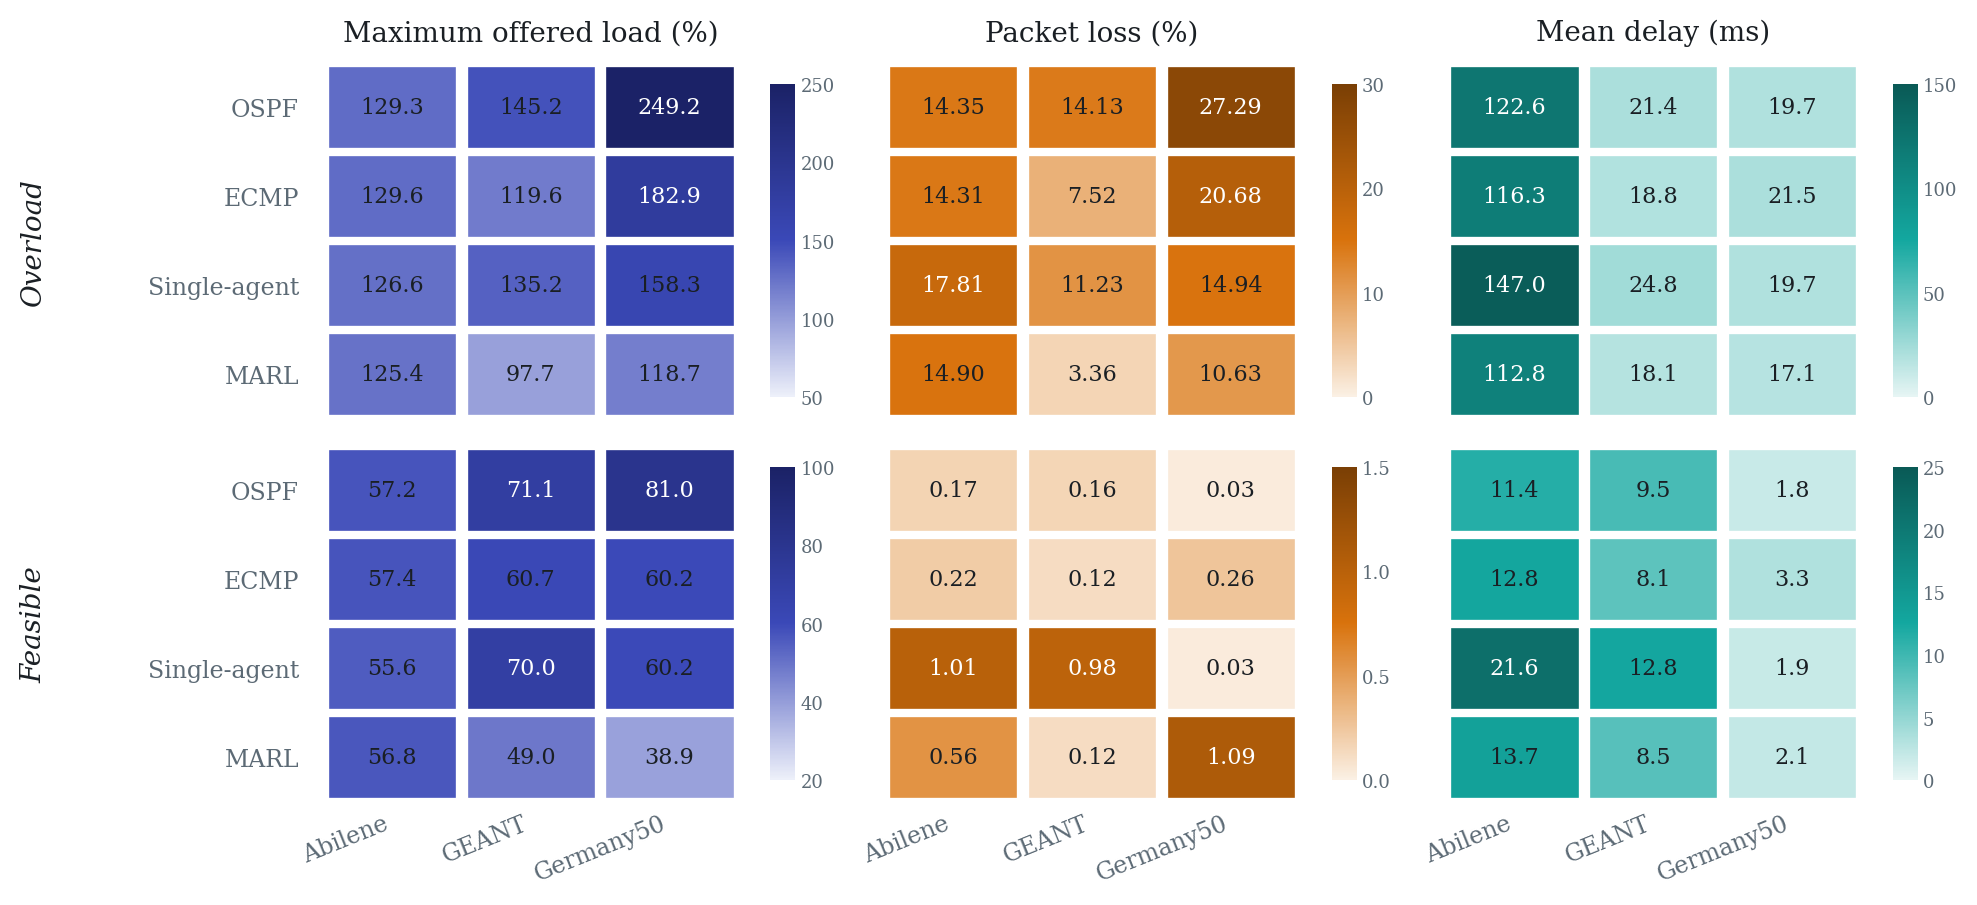
\includegraphics[width=\textwidth]{images/fig_heatmap_summary.png}
  \caption{Maximum offered load, packet loss and mean delay for the four methods
  on the three evaluation backbones, by congestion regime. Each metric is shaded
  within its own panel, so colour reads as distance from the best method on that
  network; absolute values are printed in every cell. Means over three model
  seeds.}
  \label{fig:heatmap}
\end{figure}

\subsection{Reward Trade-offs on Unseen Topologies}
\label{sec:res-reward}

The policy was trained on seventeen SNDLib topologies across three random seeds and then evaluated on three previously unseen topologies: Abilene, GÉANT, and Germany50 (training convergence is reported in Appendix~\ref{app:training}). The objective of this evaluation was to assess the trade-offs between performance gains and associated costs when applying the policy to new networks; Table~\ref{tab:reward-decomp} decomposes the resulting return into its congestion and delay terms. On Abilene, the policy detours on only $3.0\%$ of hops, incurs a cost of $4.8$, and reduces the bottleneck to $96\%$ of OSPF's bottleneck. On GÉANT, the policy detours on $3.8\%$ of hops, with a cost of $8.4$, reducing the bottleneck to $67\%$ of OSPF's. On Germany50, the largest improvement is observed, with the bottleneck reduced to $47\%$ of OSPF's, at the expense of detouring on $14.2\%$ of hops and a cost of $61.0$.

The trade is struck very differently across the three networks. On Abilene and GÉANT the return is dominated by the congestion term and the delay penalty is small, but on Germany50 the delay penalty is the larger of the two: the policy achieves its best bottleneck reduction there, to $47\%$ of OSPF's, yet pays enough detour hops that its overall return falls below the $-100$ that OSPF scores by construction. Lower bottleneck utilization is therefore not free.

These results indicate that the policy can be applied to other networks. Evaluation on previously unseen topologies demonstrates the trade-offs associated with the method employed in this study. Additional training with more steps, diverse topologies, and varied traffic patterns may further enhance model performance.

\subsection{Bottleneck Offered Load}
\label{sec:res-util}

Measured traffic data from SNDLib \citep{SNDlib10} provides actual traffic values across multiple timeframes. Traffic scaling is applied to generate demand for simulation. The resulting load is simulated on an analytical surrogate domain, since ns-3 link capacity is limited to 100\%. Therefore, simulation demand is evaluated under two distinct conditions: overload and feasible regimes. Results for both regimes are reported for all three networks.

Figure~\ref{fig:link-utilization} breaks the offered-load panel of Figure~\ref{fig:heatmap} out by topology, with the underlying values listed in Table~\ref{tab:offered-util}. The results show that MARL consistently outperforms other methods in both overload and feasible regimes. MARL achieves superior performance compared to OSPF, ECMP, and single-agent approaches on the GEANT and Germany50 networks, although it performs slightly worse than the single-agent method on Abilene. Additionally, MARL demonstrates a significant reduction in maximum offered load, achieving up to a 53\% decrease on GEANT and Germany50 in both regimes. In the overload regime, MARL reduces the offered load to 96.6\%, maintaining it below the 100\% threshold.

In the feasible regime, OSPF reaches a maximum offered load of 81\% on Germany50, while ECMP achieves 70.4\%. ECMP's more efficient algorithm results in approximately an 11\% reduction on both GEANT and Germany50 in the feasible regime. The single-agent approach shows significant improvement on Germany50 at 52\%, but underperforms on GEANT at 70\%. MARL outperforms all three baselines on GEANT and Germany50, achieving 48.2\% and 40.9\%, respectively.

The overload regime yields results similar to those observed in the feasible regime. Both the single-agent and MARL approaches improve routing decision performance in this regime. The single-agent method outperforms OSPF and ECMP on Abilene and Germany50, with improvements of 10\% and 29\%, respectively. MARL also demonstrates significant improvement by reducing the maximum offered load on GEANT and Germany50 to 96.6\% and 117\%, respectively.

These observations demonstrate that MARL improves routing by reducing the maximum offered load across both overload and feasible regimes. MARL also outperforms the single-agent approach on GEANT and Germany50. In two out of three networks, across both regimes, MARL distributes traffic more effectively than OSPF, ECMP, and single-agent methods. Therefore, the objective of using MARL to lower the bottleneck achieved.  



\begin{figure}[htbp]
  \centering
  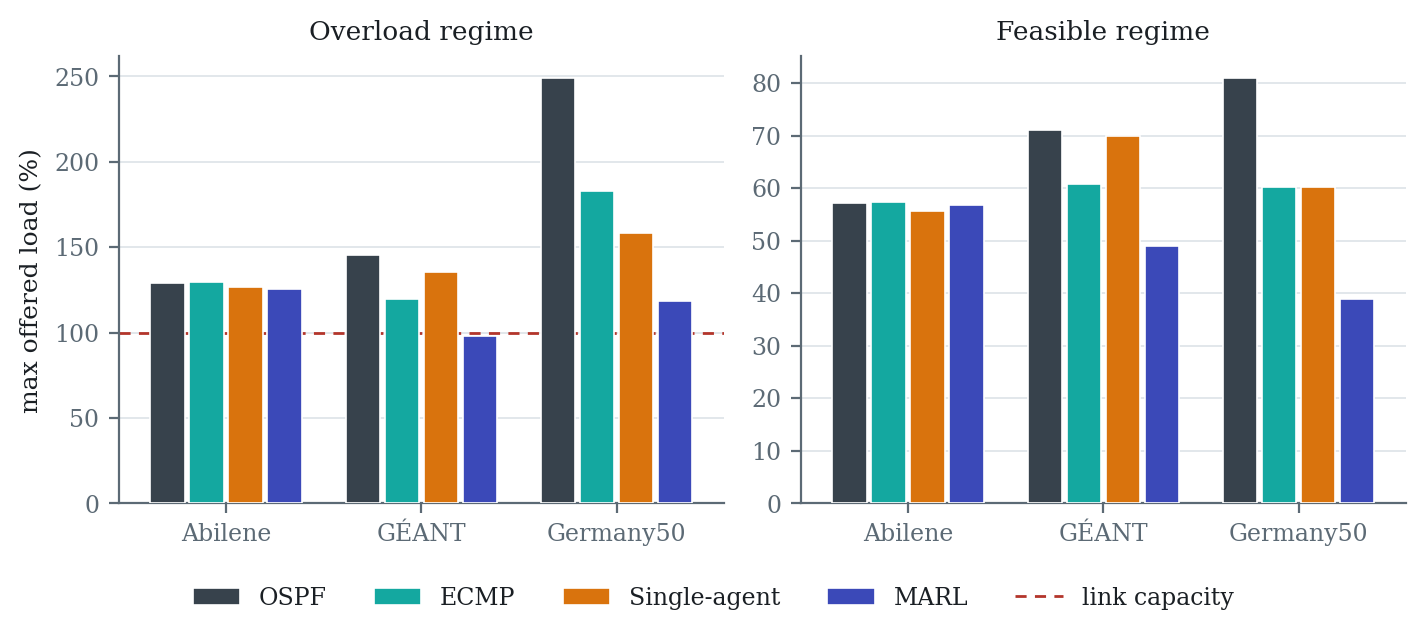
\includegraphics[width=0.8\textwidth]{images/fig_offered_util_regime.png}
  \caption{Maximum offered load on the bottleneck link, by regime and topology.}
  \label{fig:link-utilization}
\end{figure}

% \subsection{Greedy References}
% \label{sec:res-greedy}

% Neither learned policy should be credited with what a simple heuristic on the same
% action space already achieves. Table~\ref{tab:greedy} scores the two greedy
% best-responses of Section~\ref{sec:setup-hyper} on the identical matrices. Both
% require global link state after every decision and the path-level variant requires
% the demand matrix in advance, so neither is deployable; they are bounds, not
% competitors.

% \begin{table}[htbp]
%   \centering
%   \small
%   \caption{Greedy best-responses against OSPF and the reported learned arms, as
%   maximum offered load (\%). The path-level greedy shares the centralized action
%   space, the hop-level greedy the decentralized one.}
%   \label{tab:greedy}
%   \setlength{\tabcolsep}{4.5pt}
%   \begin{tabular}{lccccc}
%     \toprule
%     Cell & OSPF & Greedy (hop) & Greedy (path) & Single-agent & MARL $h{=}32$ \\
%     \midrule
%     Abilene overload   & 129.3 & 403.8 & \textbf{111.3} & 116.3 & 124.9 \\
%     GÉANT overload     & 145.2 & 148.8 & \textbf{87.9}  & 133.7 & 96.6  \\
%     Germany50 overload & 249.2 & 168.5 & \textbf{116.4} & 176.3 & 117.0 \\
%     \midrule
%     Abilene feasible   & 57.2  & 182.2 & \textbf{49.4}  & 54.2  & 56.1  \\
%     GÉANT feasible     & 71.1  & 72.4  & \textbf{45.7}  & 70.0  & 48.2  \\
%     Germany50 feasible & 81.0  & 56.8  & \textbf{37.7}  & 52.3  & 40.9  \\
%     \bottomrule
%   \end{tabular}
% \end{table}

% The two references separate sharply, and the separation is informative.

% \emph{Acting greedily hop by hop is far worse than not trying at all.} The
% hop-level best-response is beaten by OSPF on four of six cells and is
% catastrophic on Abilene, reaching $403.8\%$ where OSPF sits at $129.3\%$: choosing
% the locally least-congested next hop repeatedly walks a demand into a long path
% that loads links no single decision was accountable for. That the decentralized
% policy, acting in exactly this space, instead reaches $124.9\%$ and $96.6\%$ is
% the clearest evidence in this chapter that it has learned something beyond
% greed --- on GÉANT overload it improves on greedy by $52$ percentage points, and
% on Abilene by $279$.

% \emph{Acting greedily over whole paths is very strong.} The path-level
% best-response is the best arm in every cell, and by margins that are not small on
% GÉANT ($87.9$ against MARL's $96.6$) and Abilene ($111.3$ against the centralized
% policy's $116.3$). Only on Germany50 does a learned policy match it, MARL reaching
% $117.0$ against $116.4$. This bounds the contribution honestly: at $50$ nodes the
% learned policy is at the ceiling that its action space permits, while at $22$ and
% $12$ nodes a clairvoyant heuristic still does better. The gap is not evidence that
% the policies are under-trained --- they are at a matched budget and their seeds
% agree --- but that a policy acting on local observations, without the demand matrix
% and without recomputing global state per decision, pays something for that
% restriction. What it buys in exchange is the ability to run at all in a real
% network, where neither greedy reference could.

\subsection{Packet-Level Quality of Service}
\label{sec:res-qos}
Quality of Service results were obtained using the NS-3 simulator. FlowMonitor was employed to collect data from this packet-level simulator. To ensure consistency, measured traffic from SNDLib was used under maximum offered load conditions. The results are divided into overload and feasible regimes to highlight differences between these conditions. Packet loss is reported as a percentage, and delay is measured in milliseconds (ms). Table~\ref{tab:qos} lists the complete set of packet-level measurements, and Figures~\ref{fig:loss-qos} and~\ref{fig:delay-qos} break the corresponding panels of Figure~\ref{fig:heatmap} out by topology.

Overall, MARL is the strongest method in the overload regime, leading on four of the six loss and delay measurements. It achieves the lowest packet loss and delay at GEANT and demonstrates superior delay performance at Abilene and packet loss at Germany50. MARL reduces packet loss to 2.92\% at GEANT. However, as shown in Figure \ref{fig:loss-qos} and Figure \ref{fig:delay-qos}, loss and delay results are similar across methods in the feasible regime, with both MARL and ECMP achieving a packet loss of 0.12\% at GEANT.

MARL demonstrates strong performance in the overload regime by outperforming other methods in four out of six metrics. Specifically, it reduces delay to 108.8 ms at Abilene and 18.1 ms at GEANT under bottleneck traffic conditions. MARL also achieves the lowest packet loss at Germany50, with a value of 10.62\%. In contrast, the single-agent method achieves the lowest packet loss at Abilene (13.41\%), and ECMP achieves the lowest delay at Germany50 (17 ms).

In contrast, results in the feasible regime do not indicate significant differences in quality of service among the methods. Several metrics are identical across topologies and methods. For example, OSPF and ECMP both achieve a delay of 11.5 ms at Abilene, ECMP and MARL both record a packet loss of 0.12\% at GEANT, and OSPF and the single-agent method both achieve a packet loss of 0.03\% at Germany50. In this regime, packet loss varies only between 0.03 and 1.02\%, and delay ranges from 1.8 to 14.2 ms.

Quality of Service measurements demonstrate that MARL provides improved performance in the overload regime. The observed delay and packet loss are influenced by the routing protocol, particularly when hops increase or bottleneck traffic occurs. The study's objective is achieved, with the additional observation that in the feasible regime, baseline protocols such as OSPF and ECMP already provide sufficient performance.

\begin{figure}[htbp]
  \centering
  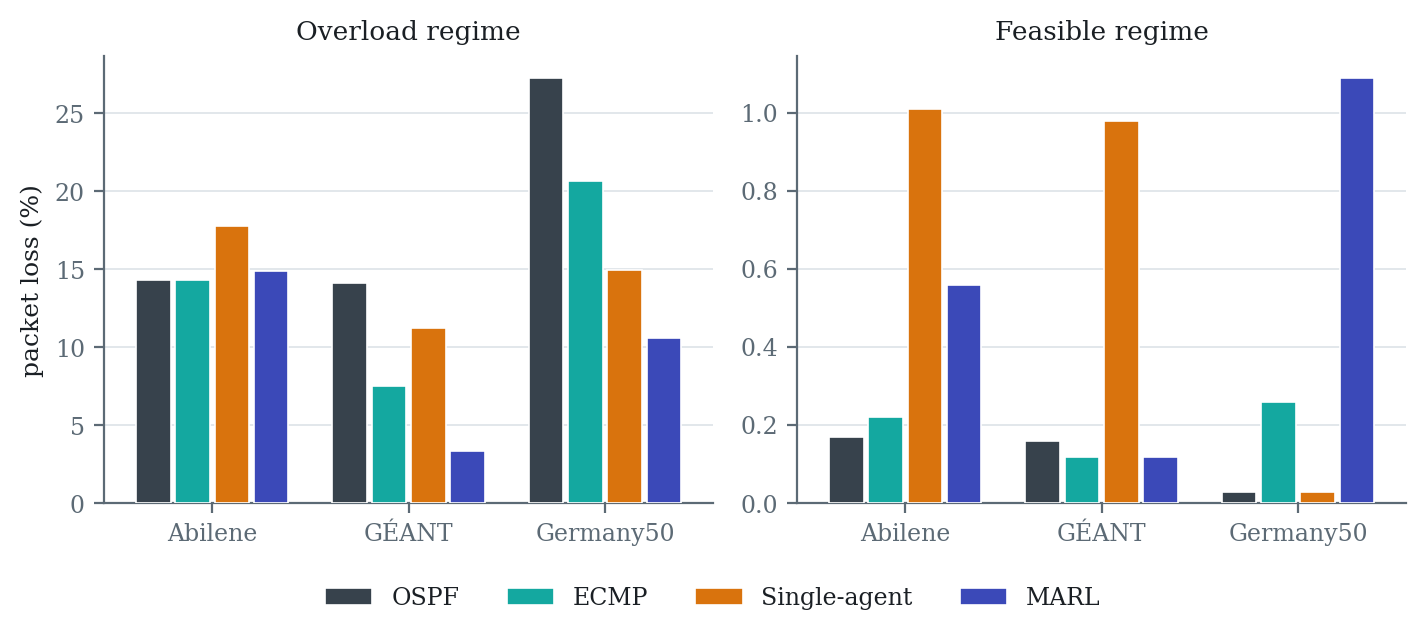
\includegraphics[width=0.8\textwidth]{images/fig_qos_loss_regime.png}
  \caption{Packet loss measured by ns-3 FlowMonitor, split by regime.}
  \label{fig:loss-qos}
\end{figure}

\begin{figure}[htbp]
  \centering
  
\includegraphics[width=0.8\textwidth]{images/fig_qos_delay_regime.png}
  \caption{Mean end-to-end delay measured by ns-3 FlowMonitor, split by regime.}
  \label{fig:delay-qos}
\end{figure}

% \subsection{Seed Stability and the Architectural Comparison}
% \label{sec:res-stability}

% Because all four learned arms now share identical PPO hyperparameters, the
% dispersion across seeds is a property of the architecture. The centralized policy
% is markedly the less stable of the two on the largest network: $\pm 51.4$
% percentage points of offered load on Germany50 against $\pm 3.5$ for MARL at
% $h{=}32$, and $\pm 5.90$ percentage points of packet loss against MARL's
% $\pm 2.91$. Inspection of the individual seeds shows the mechanism: one
% centralized seed collapses onto shortest-path selection, choosing the
% cost-shortest of the $k=3$ candidates for almost every demand, which reproduces
% OSPF and inflates the mean without inflating the training return. Across the
% evaluation networks the centralized policy routes $62$--$95\%$ of demands on
% exactly the OSPF path, against $47$--$80\%$ for MARL, so the collapse is a matter
% of degree rather than an all-or-nothing failure. The decentralized policy, whose
% per-node action space is re-entered at every hop and whose deviations are
% therefore incremental rather than committing a whole path, is the more stable at
% scale. On Abilene the ordering reverses and the centralized policy is the tighter
% of the two ($\pm 0.82$ against $\pm 2.13$ points of loss), which is consistent
% with it being the stronger arm there.

% This reverses the expectation that a $50$-node network would be hardest for a
% decentralized learner through multi-agent credit assignment, with each agent's
% return depending on forty-nine others whose policies change concurrently. That
% effect is real but is evidently not the binding constraint at this scale: MARL is
% the stronger architecture on Germany50 under overload by $7.6$ to $9.3$ points of
% loss. What survives of the scale argument is confined to the feasible regime,
% where hop-by-hop construction produces routes that free headroom at a small but
% consistent cost in loss, and where the centralized formulation's global view of a
% whole path is the better tool.

% The reported width, $h{=}32$, was selected on the \emph{training} topologies
% (Section~\ref{sec:setup-hyper}) and not on any evidence in this chapter. A wider
% $h{=}64$ variant was trained and evaluated identically as the alternative
% candidate; it was not selected and is not reported. Its behaviour is consistent
% with the choice: it carries roughly three times the seed dispersion of $h{=}32$
% ($\pm 3.0$ against $\pm 1.6$ on GÉANT overload, $\pm 9.7$ against $\pm 3.5$ on
% Germany50) and is the only configuration tested that is worse than OSPF on any
% cell.

% Against the centralized controller the two architectures split the six cells
% evenly. MARL takes both GÉANT cells and Germany50 overload --- the three in which
% the network is large or the demand heavy --- by $8.5$, $27.7$ and $7.6$ points
% respectively. The centralized controller takes both Abilene cells and Germany50
% feasible, the three in which OSPF is already close to optimal and the useful
% deviations are few. The pattern is consistent with the mechanism argued above:
% incremental per-hop diversification pays when there is slack to redistribute, and
% whole-path selection pays when only a handful of targeted changes are worth
% making.

% That split is worth reading alongside the parameter counts of
% Table~\ref{tab:hyper}. The reported decentralized policy carries $17{,}570$
% trainable parameters against the centralized controller's $268{,}420$, a factor
% of fifteen. Whatever advantage the decentralized formulation confers where it
% wins, it is not bought with capacity.

% \subsection{Where the Decentralized Method Fails: Abilene}
% \label{sec:res-abilene}

% Abilene is where the decentralized formulation loses, and it is the one network on
% which the ranking of the two learned architectures inverts. MARL at $h{=}32$
% records $0.97\%$ loss and $14.2$\,ms delay in the feasible regime against OSPF's
% $0.17\%$ and $11.5$\,ms, and $15.41\%$ loss in overload against OSPF's $14.35\%$.
% The centralized
% controller, by contrast, matches OSPF's service in the feasible regime ($0.24\%$
% loss, $13.8$\,ms) while holding the bottleneck $8.5$ points lower at $88.1\%$,
% and takes the lowest loss in the cell under overload, $13.41\%$ against OSPF's
% $14.35\%$ and ECMP's $14.30\%$.

% So the negative result is specific rather than general: \emph{learned routing}
% improves on OSPF at twelve nodes, but the hop-by-hop decentralized formulation
% does not. Two properties of the network explain the asymmetry. First, Abilene is
% the only evaluation instance with heterogeneous link capacities, fourteen links at
% $9.92$\,Gbps and one at $2.48$\,Gbps; correctly costed, OSPF prices that link at
% four and routes around it almost entirely, so the baseline is already close to
% optimal and the margin available to any optimiser is thin. Second, with only
% twelve nodes and $132$ demand pairs there is little scope for the incremental,
% per-hop diversification that is MARL's advantage on larger networks, while its
% per-hop detour penalty still accumulates. The centralized controller, choosing
% whole cost-shortest paths, expresses exactly the small number of targeted
% deviations that this network rewards.

% This bounds the contribution in a useful way. The decentralized formulation's
% value is concentrated in networks large enough, or loaded heavily enough, that
% shortest-path routing leaves genuine slack on the table: it wins by $11.2$ points
% of loss at twenty-two nodes and by $8.6$ at fifty, and loses by roughly one point
% at twelve. The crossover lies below the scale of any of the three backbones
% studied, which is a more informative statement than a uniform win would have been.



% \subsection{Limitations}
% \label{sec:res-limitations}

% Six limitations qualify these results.

% The policies are trained against an analytical link-utilisation surrogate rather
% than ns-3, since packet-level simulation is too slow inside a training loop. The
% agreement between objective and measurement in the overload regime shows the
% surrogate is adequate there, but it does not guarantee untested regimes, and the
% Germany50 feasible cell is precisely a case where the surrogate's ranking and the
% packet-level ranking disagree.

% The Germany50 OSPF baseline is sensitive to equal-cost tie-breaking. Germany50's
% links are of uniform capacity, so weighting the metric does not change any path
% cost; it changes only which of several equal-cost paths the shortest-path
% computation returns. That choice alone moves OSPF's measured overload loss by
% several percentage points, and it moves in the direction that flatters the
% learned policies. The Germany50 margins should be read with this in mind.

% The reward comparison of Section~\ref{sec:res-reward} was run for the
% centralized architecture only. Whether the decentralized policy would likewise
% improve under the centralized reward form was not tested, so the claim is that
% the reported baseline is the stronger of two configurations, not that it is
% optimal.

% Three seeds is few, particularly given the dispersion documented in
% Section~\ref{sec:res-stability}. The Germany50 feasible utilisation figures carry
% seed standard deviations between $\pm 13$ and $\pm 20$ percentage points, and
% differences between arms within that cell are not resolved by this evidence.

% Abilene's two tables describe the same policies at different operating points, for
% the reason given in Section~\ref{sec:setup-scaling}, and should not be read
% across. Similarly, the absolute Germany50 figures correspond to the top $200$ of
% $2450$ demand pairs; all methods see the identical flow set, so the comparison is
% unbiased, but the magnitudes are those of that subset.

% Finally, topologies are static and each simulation holds a single traffic matrix.
% Link and node failures, convergence during a topology change, and adaptation to
% traffic shifting \emph{within} an episode are not evaluated. The study
% demonstrates generalisation across networks and across matrices, not adaptation
% within one, and this remains the largest gap between the present work and a
% deployable system.
 
% \input{Broader Impact}
\section{Conclusions and Future Work}
The evaluation establishes that a single Multi-Agent Reinforcement Learning (MARL) policy can generalize to previously unseen network backbones and enhance the deployed baseline at the packet level. This policy is trained using an analytical model and evaluated at the packet level. The research shows that multi-agent reinforcement learning combined with a graph neural network (GNN) routing protocol outperforms existing routing protocols such as OSPF and single-agent policies. In overload scenarios, the policy reduced packet loss from 14.1\% to 3.4\% on GÉANT and from 27.3\% to 10.6\% on Germany50 compared to OSPF. Furthermore, the results show that MARL with GNN achieves superior performance on medium to large networks, such as GEANT and Germany50. However, on the smallest topology, it does not reduce packet loss below OSPF. In the feasible range, the extra headroom comes at the cost of a slight increase in packet loss.

For future work, we recommend training the model at larger scales with packet-level data and evaluating more network topologies and traffic patterns. We also suggest extending the experiments and increasing compute power to achieve comprehensive results. In addition, this study used the actor-critic Proximal Policy Optimization algorithm for rewards, so other algorithms could be explored in the future. Testing the model on real hardware routers could also help move toward a production-ready model.


\bibliography{main}
\bibliographystyle{tmlr}

\appendix
\section{Additional Tables}
\label{app:instances}

\begin{table}[h]
\centering
\small
\caption{Evaluation instances and protocol.}
\label{tab:eval-setup}
\begin{tabular}{lccc}
\hline
& Abilene & GEANT & Germany50 \\
\hline
Nodes $N$ & $12$ & $22$ & $50$ \\
Links $|\mathcal{E}|$ (undirected) & $15$ & $36$ & $88$ \\
Link capacities (Gb/s) & $9.92\ (\times 14),\ 2.48\ (\times 1)$ & $40$ & $40$ \\
Propagation delay range (ms) & $0.66$--$10.96$ & $0.58$--$33.98$ & $0.13$--$1.26$ \\
Demand pairs $|\mathcal{D}|$ & $132$ & $462$ & $2450$ \\
Pairs carried in ns-3 & all & all & top $200$ \\
Demand granularity & $5$\,min & $15$\,min & $5$\,min \\
\hline
Demand scales $\mathcal{Z}$ (analytical) & $\{8,12,16\}$ & $\{3,5,7\}$ & $\{35,50,65\}$ \\
Demand scales $\mathcal{Z}$ (packet-level) & $\{16,22,28\}$ & $\{3,5,7\}$ & $\{15,\dots,30\},\{35,50,65\}$ \\
Candidate matrices per scale & $6$ & $6$ & $6$ \\
Matrices retained per regime & $3$ & $3$ & $3$ \\
\hline
\end{tabular}
\end{table}




\begin{table}[htbp]
  \centering
  \small
  \caption{Maximum offered load. Mean $\pm$ standard deviation over ten model seeds.}
  \label{tab:offered-util}
  \setlength{\tabcolsep}{4.5pt}
  \begin{tabular}{lcccc}
    \toprule
    Topology & OSPF & ECMP & Single-agent & MARL  \\
    \midrule
    \multicolumn{5}{l}{\emph{Overload regime (OSPF drives a link $\geq$ capacity)}} \\
    \midrule
    Abilene   & 129.3\% & 129.6 $\pm$ 0.4\% & 126.6 $\pm$ 11.2\% & \textbf{125.4 $\pm$ 3.0\%}          \\
    GÉANT     & 145.2\% & 119.6 $\pm$ 10.1\% & 135.2 $\pm$ 21.5\%         & \textbf{97.7 $\pm$ 2.6\%}  \\
    Germany50 & 249.2\% & 182.9 $\pm$ 26.4\% & 158.3 $\pm$ 35.7\%         & \textbf{118.7 $\pm$ 9.6\%}         \\
    \midrule
    \multicolumn{5}{l}{\emph{Feasible regime (traffic fits under OSPF)}} \\
    \midrule
    Abilene   & 57.2\% & 57.4 $\pm$ 0.1\% & \textbf{55.6 $\pm$ 2.5\%} & 56.8 $\pm$ 2.1\%           \\
    GÉANT     & 71.1\% & 60.7 $\pm$ 5.5\% & 70.0 $\pm$ 12.0\%          & \textbf{49.0 $\pm$ 0.9\%}  \\
    Germany50 & 81.0\% & 60.2 $\pm$ 9.2\% & 60.2 $\pm$ 13.5\%         & \textbf{38.9 $\pm$ 2.6\%}         \\
    \bottomrule
  \end{tabular}
\end{table}

\begin{table}[htbp]
  \centering
  \small
  \caption{Quality of Service Results. Mean $\pm$ standard deviation over ten model
  seeds. Utilization is reported only in the feasible regime, since under overload
  every method saturates the bottleneck link at $100\%$.}
  \label{tab:qos}
  \setlength{\tabcolsep}{3.5pt}
  \begin{tabular}{llcccc}
    \toprule
    Topology & Metric & OSPF & ECMP & Single-agent & MARL \\
    \midrule
    \multicolumn{6}{l}{\emph{Overload regime}} \\
    \midrule
    \multirow{2}{*}{Abilene}   & Loss  & 14.35\%   & \textbf{14.31 $\pm$ 0.02\%}                     & 17.81 $\pm$ 4.67\% & 14.90 $\pm$ 1.69\%\\
                               & Delay & 122.6\,ms & 116.3 $\pm$ 4.4\,ms                   & 147.0 $\pm$ 24.4\,ms  & \textbf{112.8 $\pm$ 8.2\,ms} \\
    \cmidrule(l){1-6}
    \multirow{2}{*}{GÉANT}     & Loss  & 14.13\%  & 7.52 $\pm$ 2.41\%             & 11.23 $\pm$ 4.54\%          & \textbf{3.36 $\pm$ 0.69\%} \\
                               & Delay & 21.4\,ms & 18.8 $\pm$ 1.6\,ms           & 24.8 $\pm$ 6.2\,ms          & \textbf{18.1 $\pm$ 1.6\,ms} \\
    \cmidrule(l){1-6}
    \multirow{2}{*}{Germany50} & Loss  & 27.29\%  & 20.68 $\pm$ 2.83\%             & 14.94 $\pm$ 4.97\%  & \textbf{10.63 $\pm$ 2.63\%} \\
                               & Delay & 19.7\,ms & 21.5 $\pm$ 5.7\,ms            & 19.7 $\pm$ 2.2\,ms  & \textbf{17.1 $\pm$ 4.6\,ms}   \\
    \midrule
    \multicolumn{6}{l}{\emph{Feasible regime}} \\
    \midrule
    \multirow{3}{*}{Abilene}   & Loss  & \textbf{0.17\%}   & 0.22 $\pm$ 0.04\%             & 1.01 $\pm$ 1.65\%   & 0.56 $\pm$ 0.67\%   \\
                               & Delay & \textbf{11.5\,ms} & 12.8 $\pm$ 1.3\,ms           & 21.6 $\pm$ 16.2\,ms  & 13.7 $\pm$ 3.7\,ms  \\
                               & Util  & 96.7\%            & 96.8 $\pm$ 0.1\%             & \textbf{91.4 $\pm$ 5.2\%} & 92.4 $\pm$ 3.7\% \\

    \cmidrule(l){1-6}
    \multirow{3}{*}{GÉANT}     & Loss  & 0.16\%   & \textbf{0.12 $\pm$ 0.00\%}            & 0.98 $\pm$ 2.04\%   & \textbf{0.12 $\pm$ 0.00\%}  \\
                               & Delay & 9.5\,ms  & \textbf{8.1 $\pm$ 0.1\,ms}           & 12.8 $\pm$ 4.0\,ms  & 8.5 $\pm$ 0.3\,ms \\
                               & Util  & 97.3\%   & 79.4 $\pm$ 7.7\%                      & 90.5 $\pm$ 9.0\%    & \textbf{66.3 $\pm$ 1.4\%} \\

    \cmidrule(l){1-6}
    \multirow{3}{*}{Germany50} & Loss  & \textbf{0.03\%}  & 0.26 $\pm$ 0.35\%             & \textbf{0.03 $\pm$ 0.00\%} & 1.09 $\pm$ 0.83\% \\
                               & Delay & \textbf{1.8\,ms} & 3.3 $\pm$ 2.2\,ms            & 1.9 $\pm$ 0.1\,ms          & 2.1 $\pm$ 0.2\,ms \\
                               & Util  & 95.6\%           & 71.6 $\pm$ 11.3\%            & 69.6 $\pm$ 14.0\%          & \textbf{65.5 $\pm$ 16.1\%} \\

    \bottomrule
  \end{tabular}
\end{table}






\end{document}
